\scanpage{29}

% L1–9 top
\deleted{\uline{Prop.} Les \deleted{\unsure{3 bases|bitriades}} \inserted{parties 3-libres} ordonnées sont conjuguées. Si}

\deleted{$J$ est une telle partie, $\exists$ exactement deux bases qui la contiennent, soit $I$ et $I'$, et $\underbrace{(I-J)}_{K}\cup\underbrace{(I'-J)}_{K'}$ est de cardinal 6, et formé de l'ens des \unsure{$\delta$ de $S$|$\delta\in\Delta-J$} qui ne sont liés à aucun él. de $K$. De plus, $\exists!$ bibase $I\cup I'$ contenant $K\cup K'$, et $K,K'$ sont respect\textsuperscript{t} les int. de $I,I'$ avec $K\cup K'$, et \deleted{\unsure{ils sont conjugués}} \inserted{$\exists$ donc \unsure{$K\cup K'$ est stable}}, \deleted{\unsure{correspondance} par \unsure{$t$|$\sigma$} (l'unique autom $\ne\mathrm{id}$ qui \unsure{ne bouge pas|respecte|fixe} la bibase \ldots)} et si}

% L10–11
\[
 \begin{aligned}
 J&=\deleted{\{\lambda_{45},\lambda_{56},\lambda_{61}\}}\\
 K\cup K'&:\ \deleted{\{\underbrace{\unsure{\zeta|\xi}_1,\zeta_2,\zeta_3}_{K},
 \underbrace{\zeta'_1,\zeta'_2,\zeta'_3}_{K'}\}}
 \end{aligned}
\]

% L12–13
\[
 \begin{aligned}
 &\deleted{6!=720=2^4\,3^2\,5}\qquad72\ \text{bases}\quad/\ \underline{36\ \text{bibases}}\\
 &\deleted{6^4=2^4\,3^4=1296}\qquad40\ \text{trihexagones}
 \end{aligned}
 \qquad\begin{array}{r}36\\36\\\hline216\\108\phantom0\\\hline1296\end{array}
\]

% L14–17 left
\[
 \begin{array}{lr}\text{sommets}&27\\\text{bibases}&36\\
 \text{trihexagones}&40\\\text{triangles}&45\end{array}
\]

% middle
\figure{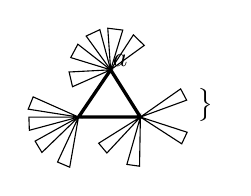
\begin{tikzpicture}[scale=.6]
\coordinate (a) at (0,1);\coordinate (b) at (-.68,0);\coordinate (c) at (.63,0);
\draw[very thick] (a)--(b)--(c)--cycle;
\foreach \ang in {36,73,105,142,183}{\draw (a)--++(\ang:.88)--++(\ang+100:.32)--cycle;}
\foreach \ang in {156,180,209,245}{\draw (b)--++(\ang:1.05)--++(\ang+92:.28)--cycle;}
\foreach \ang in {35,-18,-91,-133}{\draw (c)--++(\ang:1.04)--++(\ang-97:.27)--cycle;}
\node at (.2,1.19) {$\unsure{a}$};\node at (2,.25) {$\big\}$};
\end{tikzpicture}}

% L14–19 middle right
\[
 \begin{aligned}
 &\unsure{\mathfrak S|\mathfrak G}_4\\
 &\deleted{\unsure{4|2}}\mathfrak S_3/\mathfrak S_4/\mathbb F_2^{\unsure{3}}\\
 &72\cdot24\\&2^{\unsure{7}}\cdot9
 \end{aligned}
\]

% L18–21 lower left
$\mathfrak S_4\ \mathbb F_2^4\quad\mathrm{ord.}\quad24\cdot16$

\unsure{qui fixe|quadriques} deux droites $3$ sur $\mathbb F_2$

$8\cdot\mathrm{G\unsure{L|l}}(3,\mathbb F_2)$

$\deleted{\unsure{P(i)}}\quad\deleted{\unsure{2}}\quad 8-2/2=3$

% L18–21 lower centre
$A(i)$ ens à 4 él. \quad $i\in T$

$P(i)$ torseur sous $\unsure{V(i)|k(i)}=\mathbb F_2^{A(i)}\quad\left.\vphantom{\mathbb F_2^{A(i)}}\right\}\text{ à 16 él.)}$

$\forall i$, bijection entre $P(i)$ et $\displaystyle\coprod_{j\in T-\{i\}}\ \unsure{\alpha}\in A(j)$

% L22–26 left
\[
 \begin{aligned}
 &P(i)/\deleted{\unsure{W|V}}V'(i)\simeq T-\{i\}\\
 &(1+q)(1+q^{\unsure{2|-1}})\,q^{3}(q-1)^2\qquad q=2\\
 &2^3\cdot3\cdot5\mathbin{\unsure{=|.}}\underline{120}\ !!!\quad\deleted{P(i)}\\
 &20
 \end{aligned}
\]

% L22–26 centre
\diagram{\begin{tikzcd}[ampersand replacement=\&,column sep=small,row sep=small]
 {}\arrow[r,dash]\& k\arrow[r,phantom,"\scriptstyle\subset" description]\&V'(i)\arrow[r,phantom,"\scriptstyle\subset" description]\&V(i)\arrow[r,dash]\&0\\
 {}\arrow[r,dash]\& {}\arrow[r,dash]\& {}\arrow[r,dash]\&{}\\
 1\&2\&1
\end{tikzcd}}

% L24–27 centre
\diagram{\begin{tikzcd}[ampersand replacement=\&,execute at end picture={\begin{scope}[x=.72cm,y=.72cm]\coordinate (a) at (1.25,0);
\coordinate (b) at (1,1.3);
\coordinate (c) at (0,0);
\draw[->] (a)--(b);
\draw (a)--(c);
\draw[dashed] (b)--(c);
\fill (a) circle (1.15pt);\node[right,inner sep=1.2pt] at (a) {$a$};
\fill (b) circle (1.15pt);\node[above,inner sep=1.2pt] at (b) {$b$};
\fill (c) circle (1.15pt);\node[left,inner sep=1.2pt] at (c) {$c$};
\end{scope}}] {} \end{tikzcd}}

% L24–29 centre right
$V'(i)\quad \deleted{\unsure{V^+(i)|V'(i)}}\quad\unsure{\Gamma_i|P_i}$

$\begin{matrix}k\subset V'\\ \downarrow\\ \mathrm{Aut}(E)\end{matrix}$

% L27–30 lower right
\[
 \begin{matrix}&A_1&\\A_3&&A_2\\\multicolumn{3}{c}{\underbrace{\hspace{3em}}_{\text{3 ens. à 4 él.}}}\end{matrix}
\]

% L29–31 lower left
$V$ vectoriel de dim 3 sur $\mathbb F_2$ \unsure{et}

$\underset{\scriptscriptstyle k}{V}\simeq\underset{\scriptscriptstyle k}{K(A_i)'}$ pour tt $i$\qquad $A_3\times$

% foot right
$V\supset k$ vectoriel de dim 3 sur $\mathbb F_2$
% archive sheet number: 28
